Domain Experts are users who would use Magpie as a tool for their work. We
interviewed 3 individuals who fit this criteria. The Domain Expert test sessions
took the following format:
\begin{enumerate}
    \item \textbf{Getting to know:} this first step is designed to introduce
          ourselves to the participants, inform ourselves of their background and
          occupation and set the tone for the rest of the session.
    \item \textbf{Introduction of Magpie:} this second step serves to give an
          overview of Magpie's purpose, features, data displayed and functionalities.
    \item \textbf{Exploring Magpie + Discussion:} this third step will allow the
          participants to explore the application, ask question and reflect on how
          Magpie can be used to meet their needs for their work.
    \item \textbf{Satisfaction survey + End of session:} this last step serves
          to conclude the session by asking the participants to fill in a satisfaction
          survey to quantify their experience using Magpie.
\end{enumerate}

\subsubsection{User 7 - Bryan Boyle}
Bryan Boyle is a lecturer at the University College Cork in Occupational
Sciences and Therapy. With a doctorate in Computer Science and Occupational
Therapy, they have published several papers related to inclusivity in public
spaces (\cite{bryanboyleplaygroundinclusion2023}), and the role of technology in
the lives of individuals with disabilities
(\cite{bryanboylechildrenautism2022}).

They gave their contact information during the research survey. They are
categorized as a \emph{Domain Expert} because they utilise amenity data in their
work, and Magpie could potentially be a tool they use. Firstly, we got to know
Bryan Boyle, his professional experience and the amenity data he uses for his
research. His area of research focuses on topics of child development and
inclusivity.
%bryan amenity info
\begin{figure}[h!]
    \centering
    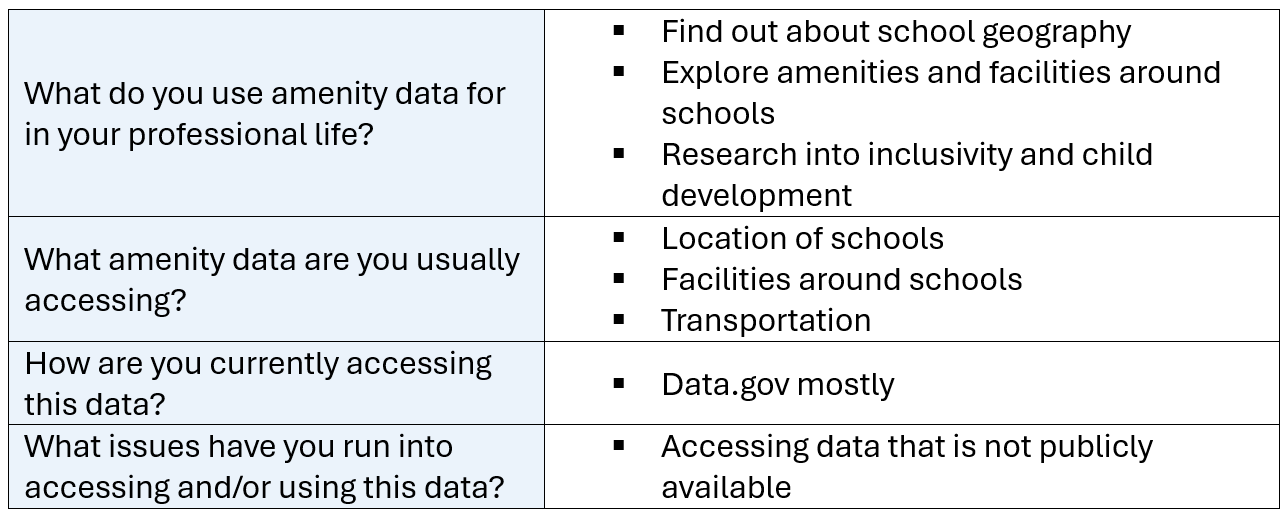
\includegraphics[width=0.9\textwidth]{images/bryan-amenity-info.png}
    \caption{User Evaluation - Bryan Boyle information}
\end{figure}

\newpage{}

\noindent Next, we introduced Magpie and started the uncontrolled session. The
approach was to guide Bryan Boyle through the homepage whilst introducing
Magpie, and then let them explore on their own while discussing their thoughts.
They were able to complete most of the general tasks, except for zooming in and
out. This is because they were not familiar with mouse scrolling, the onboarding
was not clear enough and zoom buttons were not present on the map.
%table of Bryan's general tasks
\begin{table}[h!]
    \centering
    \caption{Usability testing Tasks - Bryan}
    \begin{tabular}{|p{0.4\textwidth}|p{0.1\textwidth}|p{0.1\textwidth}|p{0.2\textwidth}|}
        \hline
        \textbf{Task}                 & \textbf{Status} & \textbf{Difficulty} & \textbf{Errors} \\
        \hline
        Load Magpie application       & Complete        & 2                   & N/A             \\
        \hline
        Sign up                       & Complete        & 1                   & N/A             \\
        \hline
        Log in                        & Complete        & 1                   & N/A             \\
        \hline
        Complete tutorial             & Complete        & 1                   & N/A             \\
        \hline
        Place cursor on map           & Pass            & 3                   & Required help   \\
        \hline
        Zoom in and out               & Fail            & 5                   & Required help   \\
        \hline
        Hold map and navigate         & Complete        & 1                   & N/A             \\
        \hline
        Adjust radius big/small       & Complete        & 1                   & N/A             \\
        \hline
        Clear marker \& radius        & Complete        & 2                   & N/A             \\
        \hline
        Deselect all amenities        & Complete        & 2                   & N/A             \\
        \hline
        Select one or more amenities  & Complete        & 1                   & N/A             \\
        \hline
        Find tutorial and exit midway & Complete        & 2                   & N/A             \\
        \hline
        Log out                       & Complete        & 1                   & N/A             \\
        \hline
    \end{tabular}
\end{table}

Here were the main takeaways from Bryan's session:
\begin{itemize}
    \item \textbf{Data: }they mainly looked at amenities related to
          accessibility such as accessible parking, public toilets, water fountains,
          etc\ldots They would like to see more data such as public transportation,
          facilities like schools, hospitals and stations. What really interests them
          is the type and quality of an amenity surrounding the specific location they
          are searching for, necessitating higher-level information to add to the
          tooltips.
          
    \item \textbf{General: }they really enjoyed using the search bar, they found
          it intuitive and quicker to use than placing a marker on the map. They are
          very interested in the project and look forward to seeing the final
          product.
          
    \item \textbf{Behaviour: } Bryan seems to have less than average proficiency
          with technology. Throughout the session, we noticed that first they used
          Edge as a browser, they got lost looking for the tab among the many windows
          they had open, their browser window was not full screen and additionally
          struggled zooming into the map.
\end{itemize}

\textbf{Overall}, Bryan found Magpie to be simple and very straightforward,
demonstrated by his \underline{5 out of 5} score for the user interface. He
would use it as a tool for his PhD research, mainly on desktop which further
solidifies our user persona and why we prioritized desktop compatibility before
mobile.

\hspace{2em}\textbf{Score breakdown: Appendix \ref{fig:bryanscore}}

\newpage{}
\subsubsection{User 8 - Dr. Sarah Rock}
Professional user Dr. Sarah Rock is a transport and urban planning specialist
with over 15 years of experience working in both the private and public sector.
As chair of the MSc in Urban Regeneration at the TU Dublin School of
Architecture, she pushes for sustainable and innovative solutions to land use
and urbanisation, specialising in accessibility planning and network design.

We recruited them through social media channels to take part in a user testing
session. They mostly use amenity data to understand an existing area that has
plans for upgrade or demolitions, as well as studying transportation routes to
plan new stops and service new areas.
%sarah amenity info
\begin{figure}[h!]
    \centering
    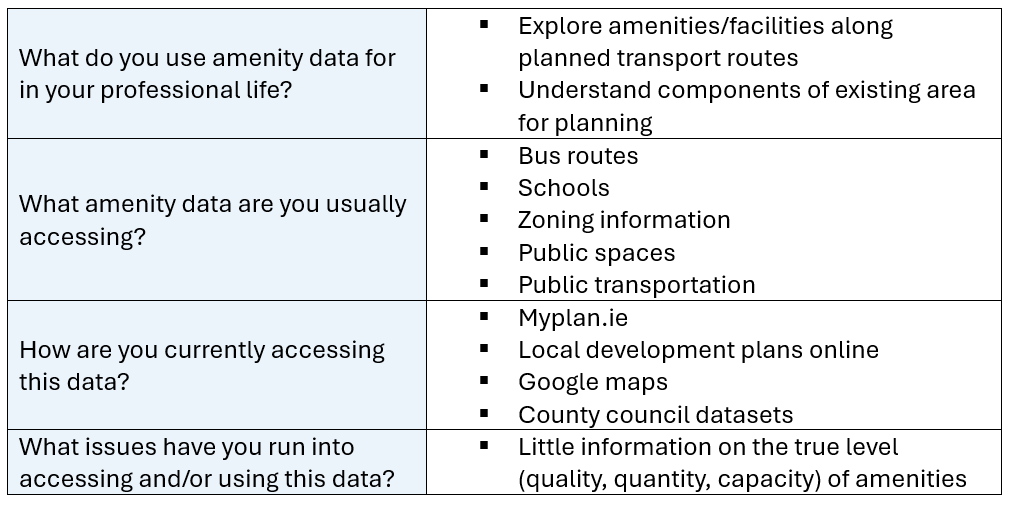
\includegraphics[width=0.8\textwidth]{images/sarah-amenity-info.png}
    \caption{User Evaluation - Dr. Sarah Rock information}
\end{figure}

\noindent Next, Dr. Rock loaded the Magpie application and started exploring,
whilst discussing each and every feature. They were able to complete all general
tasks while skipping a few. One question they asked was very interesting:
\emph{how do we define amenities?} Different professions within
urban/transport/city planning define amenities in different ways, and they found
our way of defining it interesting and slightly different from the way they
would've defined it: \emph{`Amenities are any sort of public facilities that you
    can use.'}
%table of Sarah's general tasks
\begin{table}[h!]
    \centering
    \caption{Usability testing Tasks - Dr. Sarah Rock}
    \begin{tabular}{|p{0.3\textwidth}|p{0.1\textwidth}|p{0.1\textwidth}|p{0.2\textwidth}|}
        \hline
        \textbf{Task}                 & \textbf{Status} & \textbf{Difficulty} & \textbf{Errors}                 \\
        \hline
        Load Magpie application       & Complete        & 2                   & N/A                             \\
        \hline
        Sign up                       & Pass            & 2                   & Tried to sign up on log in page \\
        \hline
        Log in                        & Complete        & 1                   & N/A                             \\
        \hline
        Complete tutorial             & Complete        & 2                   & N/A                             \\
        \hline
        Place cursor on map           & Complete        & 1                   & N/A                             \\
        \hline
        Zoom in and out               & Complete        & 1                   & N/A                             \\
        \hline
        Hold map and navigate         & Complete        & 1                   & N/A                             \\
        \hline
        Adjust radius big/small       & Complete        & 1                   & N/A                             \\
        \hline
        Clear marker \& radius        & Skipped         & N/A                 & N/A                             \\
        \hline
        Deselect all amenities        & Skipped         & N/A                 & N/A                             \\
        \hline
        Select one or more amenities  & Complete        & 1                   & N/A                             \\
        \hline
        Find tutorial and exit midway & Skipped         & N/A                 & N/A                             \\
        \hline
        Log out                       & Skipped         & N/A                 & N/A                             \\
        \hline
    \end{tabular}
\end{table}

\newpage{}

Here were the main takeaways from Dr. Rock's session:
\begin{itemize}
\item \textbf{Data:} the tooltips on each icon are very interesting. Perhaps
cross-check the information there and add/remove details. For example, the bike
sharing amenity tooltip has name, number, and address, but the number seems to
be an ID and not the number of bikes at the bike sharing station.
\vspace{0.2cm}
    \item \textbf{Additional features:} for their work, Dr. Rock likes to have a
          satellite view of the area they are inspecting. They found that when they
          are zoomed in at the street level, they find it hard to understand the map.
          Perhaps adding a satellite layer for enhanced visualisation. Also, an
          export feature would be amazing, with a scale and table of the amenities
          found on the location selected on the map.
          \vspace{0.2cm}
          
    \item \textbf{Miscellaneous:} the car parking amenity has lots of potential
          because it relates to the use of public space which is very contested and a
          big issue in urban planning. Magpie displays that information in an easy
          manner and there is so much potential to expand the parking detection and
          help fuel research on how much cars take up public space in cities and
          inefficiencies using public space for parking especially with limited land.
          
\end{itemize}

\textbf{Overall}, they stated that Magpie is a fascinating and really useful
project in its own right. The radius slider is great, the amenity count is very
useful, Dr. Rock can see Magpie being used for planning and research not so much
non-expert user. Points to improve would be more amenity data and revise the
information on the amenity tooltips. They scored Magpie's UI a \underline{4.6
    out of 5}, the tutorial and the filters losing a star for lack of clarity and
intuitiveness.

\hspace{2em}\textbf{Score breakdown: Appendix \ref{fig:sarahscore}}

\newpage{}

\subsubsection{User 9 - Odran Reid}
Odran Reid has over 30 years of experience in the public,
private and NGO sector in Europe. With degrees in economics from Trinity and
spatial planning from TU Dublin, they specialise in retail planning,
socio-economic analysis and community consultation for local development
projects. They are currently a lecturer in spatial planning at the TU Dublin
School of Architecture. We recruited them through social media channels to take
part in a user testing session. They mostly use amenity data for socio-economic
research and consulting for community project developments.

%odran amenity info
\begin{figure}[h!]
    \centering
    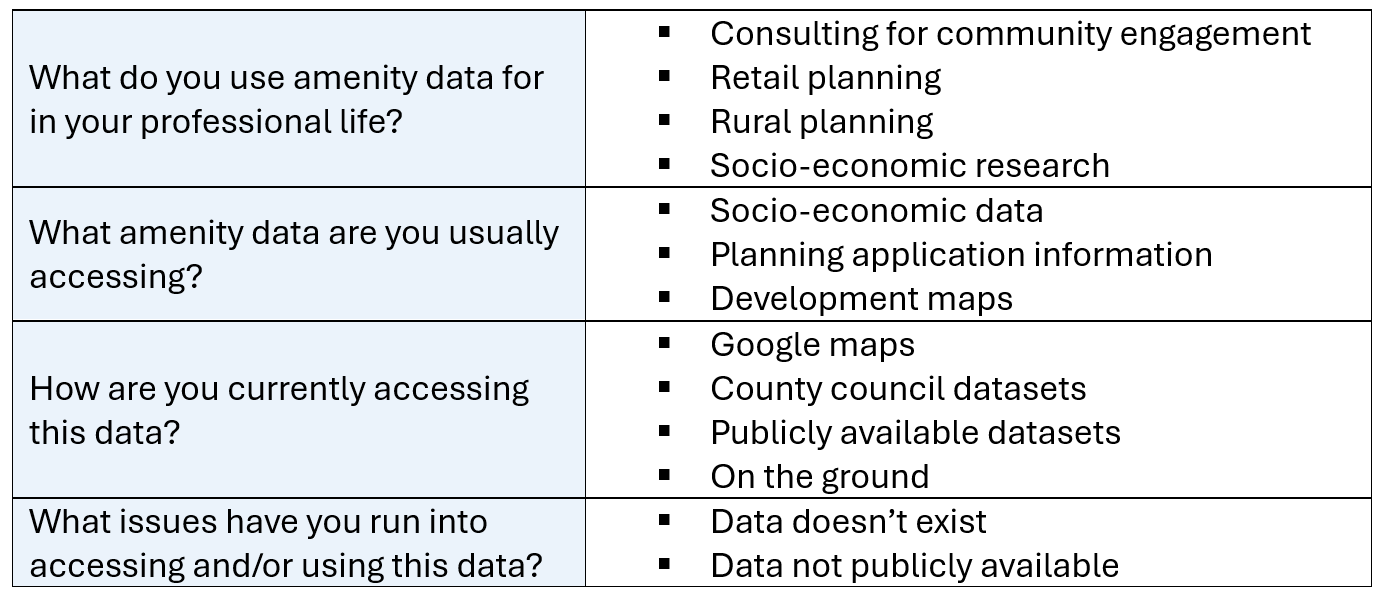
\includegraphics[width=0.8\textwidth]{images/odran-amenity-info.png}
    \caption{User Evaluation - Odran Reid information}
\end{figure}

Before the session started, Odran Reid told us they qualified their
technological proficiency as `very low' and to be patient with him. This was
confirmed when he struggled to share his screen at the start of the session,
however he was very comfortable navigating the map, zooming in and out and using
the features of the dashboard. Here were the main takeaways:
\begin{itemize}
    \item \textbf{Amenities:} they suggested some minor content changes related to the
          labelling of amenities, for example `library' should be `public library',
          `public wifi' should be `free public wifi' etc\ldots Also, it would be
          beneficial to differentiate the types of bike sharing system (Dublin Bikes,
          Bleeper, Moby Bikes). More data should be added like schools, public
          transportation, zoning information and vacant buildings.
          \vspace{0.2cm}
          
    \item \textbf{Features:} giving the user the chance to draw their own radius
          could be very interesting. Also, adding a `300 meters' preset for the radius
          slider would cater to planners more because of the 15 minute walkable
          rule. This rule states that 300m is a walkable distance for abled
          individuals and is used a lot in retail/town planning.
          \vspace{0.2cm}
          
    \item \textbf{Miscellaneous:} they suggested to look at \emph{POBAL} for
          more datasets relevant to our project.
          \vspace{0.2cm}
\end{itemize}
\textbf{Overall}, Odran Reid believes Magpie has commercial potential but needs
more datasets and more detail to turn this into the go-to tool for planners in
any sector. They expressed how they would've enjoyed having this tool earlier on
for their consulting work. They scored Magpie's UI a \underline{4.6 out of 5},
the log in and sign up losing a star for lack of email verification and
smoothness.

\begin{figure}[h!]
    \centering
    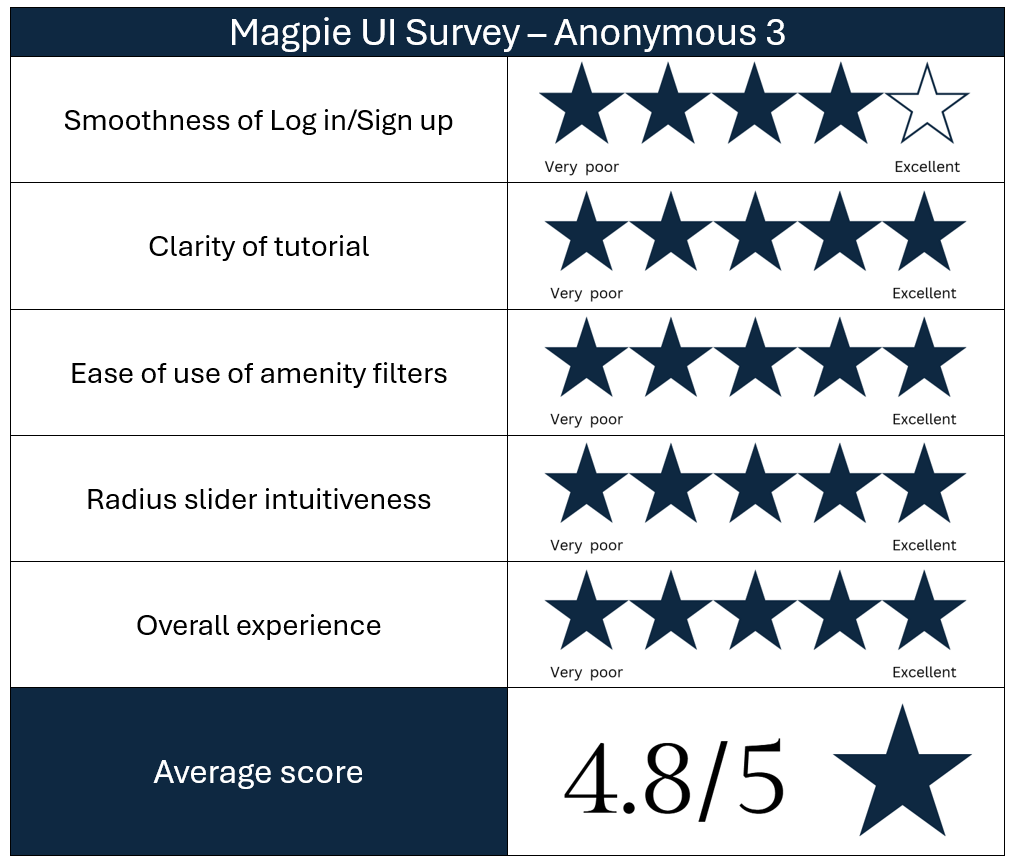
\includegraphics[width=0.7\textwidth]{images/survey-odran.png}
    \caption{User Evaluation - UI Score Odran Reid}
\end{figure}

\hspace{2em}\textbf{Score breakdown: Appendix \ref{fig:odranscore}}

\newpage{}

\subsubsection{Domain Experts overview}
Interviewing these three users was a really amazing experience. It's easy to put
all planners into one basket however, they all have different needs, experiences
and wants and these sessions really opened our eyes on that.

The main changes these users would like to see are \textbf{more data}, more
\textbf{precise information} on the amenity tooltips, an \textbf{export feature}
and improvements to the onboarding.

The scores they gave on Magpie's UI averaged to \underline{4.8 out of 5}, which
is incredible. This score validates Magpie's project vision and end goal: to
create a easy to use tool to give a glance view of amenities in an area.
%target survey response summary
\begin{figure}[h!]
    \centering
    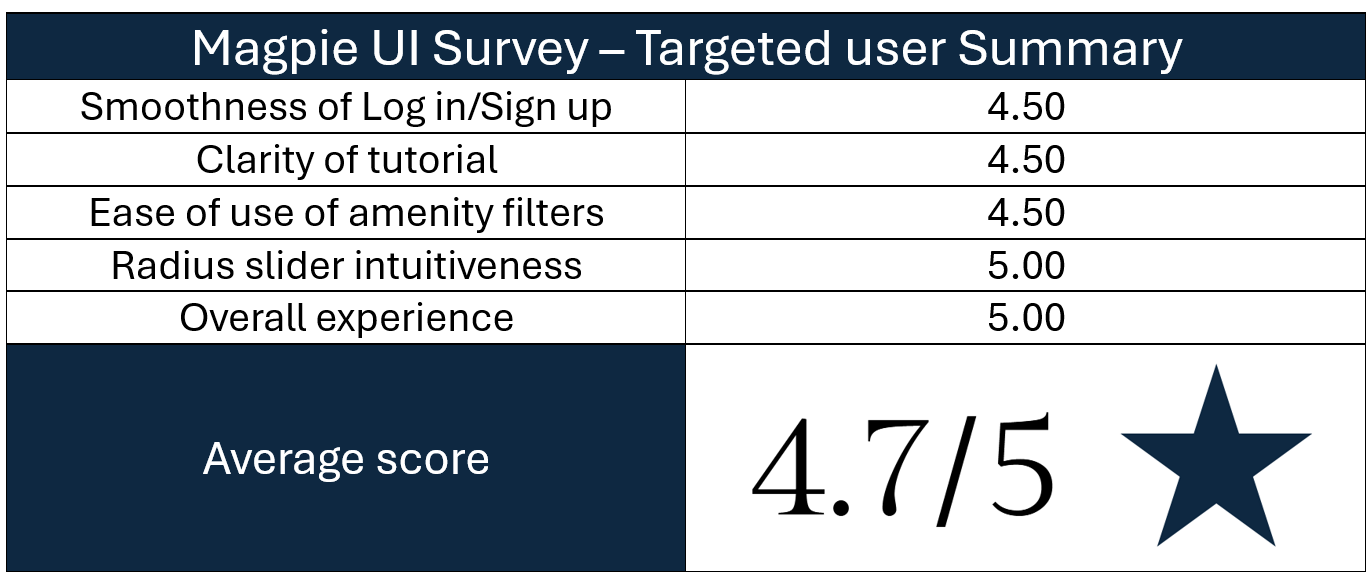
\includegraphics[width=0.7\textwidth]{images/survey-target-summary.png}
    \caption{User Evaluation - UI Target Score Average}
\end{figure}
